\section{Introduction}
Some of the material in this guide has been taken from office blog and other websites, all links are mentioned in the footnote for ease of access. The purpose of this handout is to put together necessary instructions regarding various Microsoft Word features to help you format your thesis according to the guidelines of AIT.
Let's start by setting few defaults:
\section{Setting Defaults}
\subsection{Default Font}
\begin{enumerate}
    \item Click on arrow \textbf{\emph{Font}} Group on \textbf{\emph{HOME}} Tab marked by red rectangle in the figure \ref{fig:homefont}
    \item Select Times New Roman in Font list and 12 in Size list 
    \item Click \mystyle{Set as Default} button and then Click OK in the confirmation Window
\end{enumerate}
\subsection{Page Margin and Size} 
\begin{enumerate}
\item Go to \mystyle{PAGE LAYOUT} Tab 
\item From \mystyle{Page Setup Group} Select \mystyle{Margins} and select \mystyle{Custom Margins}
\item Note that the units of measurement here if it is inches first change it to cm by following these steps:
    \begin{enumerate}
    \item Click \mystyle{FILE} and choose \mystyle{Options}
    \item Click \mystyle{Advance}
    \item Scroll down and look for \mystyle{Display} category
    \item Change \mystyle{Show measurement in units of:} to Centimeters and click OK
    \end{enumerate}
\item Now you can specify margins in centimeters, change Left margin to 3.0 cm, and 2.5 cm for Right, Top and Bottom and click OK.
\item Click \mystyle{Size} in \mystyle{Page Setup Group} group of \mystyle{PAGE LAYOUT} Tab and select \mystyle{A4}
\end{enumerate}
\begin{figure}
    \centering
    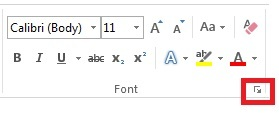
\includegraphics{./Figures/homefont.jpg}
    \caption{Font Group on Home Tab}
    \label{fig:homefont}
\end{figure}

\section{Styles}
\label{sec:styles}
Styles allow you to quickly apply a bunch of formatting such as font face, font size, font color, etc. A very detailed blog on Word Style can be read here \footnote{\url{http://blogs.office.com/2012/09/06/changing-your-style-in-the-new-word/}}. Word comes with a default style gallery, a screenshot can be seen in the figure \ref{fig:stylegallery}.
\begin{figure}[h]
    \centering
    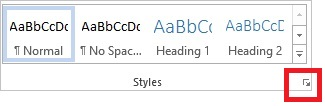
\includegraphics{./Figures/styledefine.jpg}
    \caption{Word Style Gallery}
    \label{fig:stylegallery}
\end{figure}
\subsection{Acitivity 1: Defining Style for Heading 1}
We will define the chapter title style first. It has to be bold and in capital as mentioned in the style guide \footnote{\url{http://www.languages.ait.asia/ait-style-guide/parts-of-a-thesis-2/}} 
\begin{enumerate}
    \item Click on the arrow indicated by red rectangle in the figure   \ref{fig:stylegallery}, a keyboard equivalent to this is Ctrl+Shift+Alt+S
    \item Next click the new style button indicated by rectangle in the figure \ref{fig:styletaskpane}, this will bring up the dialog to create new style shown in figure \ref{fig:chapterheading}
    \begin{figure}
        \centering
        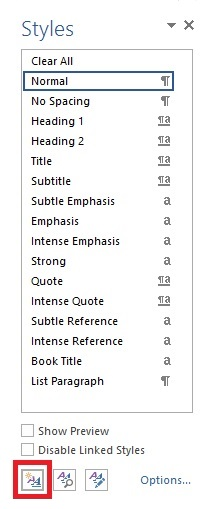
\includegraphics[scale=0.6 ]{./Figures/styletaskpane.jpg}
        \caption{New style button in Styles Gallery }
        \label{fig:styletaskpane}
    \end{figure}
    
    \item Now do the following:
    \begin{itemize}
        \item For the Name type in ChapterHeading
        \item Leave the Style type to Paragraph
        \item Leave Style based on to Normal
        \item Change Style for following paragraph to Normal
        \item From the drop down list of fonts choose Times New Roman
        \item From the size drop down choose 14
        \item Click the bold button
        \item Click the center align button
        \item Now click the Format button and choose Font
        \item Check the option for all caps and hit OK button
    \end{itemize}
    \item Finally click OK button, and you have created the first style which will be applicable to chapter heading.
    \begin{figure}
        \centering
        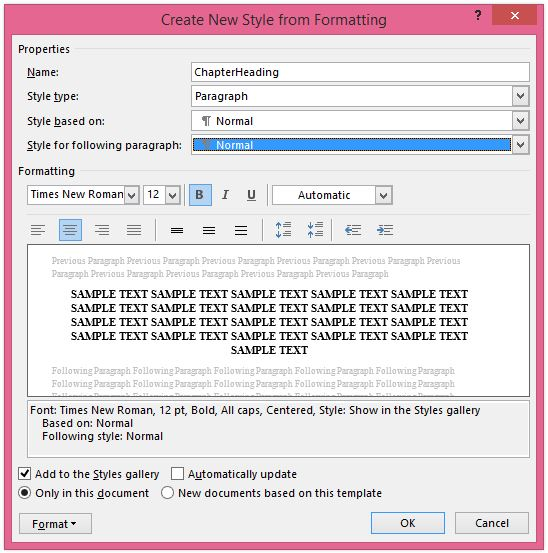
\includegraphics[scale=0.6]{./Figures/chapterheading.jpg}
        \caption{Create New Style from Formatting Dialog}
        \label{fig:chapterheading}
    \end{figure}
\end{enumerate}
    
 \subsection{Exercise 1: Do it yourself} 
 Now that you have seen how to create styles, try to create the  section heading and subsection heading styles, set the properties of the styles as given in tables \ref{tab:chaptertitle}, \ref{tab:sectionheading} and \ref{tab:subsectionheading}
 \begin{table}
     \centering
     \begin{tabular}{l | l}
         \toprule
          \multicolumn{2}{c}{Chapter Title Properties} \\ \toprule
          Name & SectionHeading \\ 
          Style type & Paragraph \\
          Style based on & Normal \\
          Style for following paragraph & Normal \\
          Font & Times New Roman \\
          Size & 14 \\
          Bold & selected \\
          Align & center \\ \bottomrule
     \end{tabular}
     \caption{Properties for Chapter Title}
     \label{tab:chaptertitle}
 \end{table}
 \begin{table}
     \centering
     \begin{tabular}{l | l}
         \toprule
          \multicolumn{2}{c}{Section Heading Properties} \\ \toprule
          Name & SectionHeading \\ 
          Style type & Paragraph \\
          Style based on & ChapterHeading \\
          Style for following paragraph & Normal \\
          Font & Times New Roman \\
          Size & 12 \\
          Bold & selected \\
          Align & left \\ \bottomrule
     \end{tabular}
     \caption{Properties for Section Heading}
     \label{tab:sectionheading}
 \end{table}
 \begin{table}
     \centering
     \begin{tabular}{l | l}
         \toprule
          \multicolumn{2}{c}{Sub Section Heading Properties} \\ \toprule
          Name & SectionHeading \\
          Style type & Paragraph \\
          Style based on & SectionHeading \\
          Style for following paragraph & Normal \\
          Font & Times New Roman \\
          Size & 10 \\
          Bold & deselect \\
          Align & left \\ \bottomrule
     \end{tabular}
     \caption{Properties for Sub Section Heading}
     \label{tab:subsectionheading}
 \end{table}
 That is all the style we need at the moment. Now Its time to integrate the styles we have created with multilevel list.
 
 \section{Multilevel lists}
 A multilevel list, as the name suggests, displays each items in the list at different level e.g. the multilevel list shown below. Notice that at each level a different format/scheme is used to specify the order of the items in the list. See \footnote{\url{https://support.office.com/en-gb/article/Create-a-multilevel-list-21a5f3cd-0be5-4319-9974-adb8cd376474}} for details.
 \begin{enumerate}
     \item Section Heading 1
         \begin{enumerate}
         \item Sub Section Heading 1 Under Section 1
         \item Sub Section Heading 2 Under Section 1
         \item Sub Section Heading 3 Under Section 1
         \end{enumerate}
     \item Section Heading 2
        \begin{enumerate}
        \item Sub Section Heading 1 Under Section 2
        \item Sub Section Heading 2 Under Section 2
        \item Sub Section Heading 3 Under Section 2
            \begin{enumerate}
            \item Sub Sub Section Heading 1 Under Section 2
            \item Sub Sub Section Heading 2 Under Section 2
            \end{enumerate}
        \end{enumerate}
 \end{enumerate}
 \subsection{Activity 2: Creating MultiLevel List and Integrating with Styles}
 We will start by defining new list style, please follow the steps below:
 \begin{enumerate}
    \item Click on the multilevel list button show in the figure, and choose "Define New List Style" \ref{fig:multilevellist}
    \begin{figure}
        \centering
        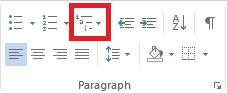
\includegraphics{./Figures/multilevellist.jpg}
        \caption{Multilevel list Button in Paragraph Group of Home Tab}
        \label{fig:multilevellist}
    \end{figure}
    \item This will bring up the dialog for new list style shown in figure \ref{fig:liststyledialog}
    \begin{figure}
    \centering
    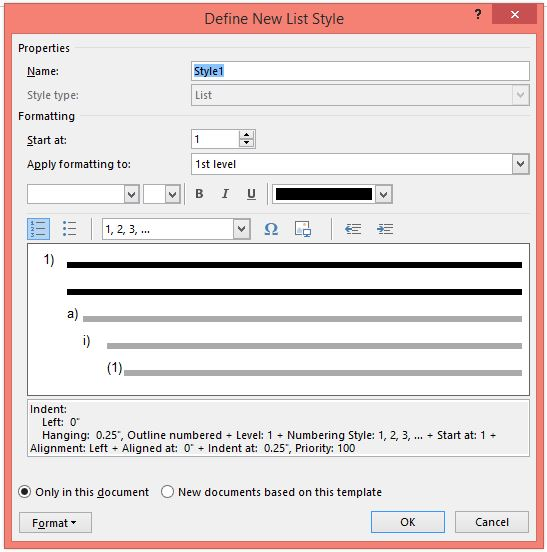
\includegraphics[width=\textwidth]{./Figures/liststyledialog.jpg}
    \caption{New List Style Dialog}
    \label{fig:liststyledialog}
    \end{figure}
    \item In the Name field for properties type AITListStyle
    \item Now Click the Format button at the bottom left of the dialog and choose Numbering
    \item Now Click the More Button at the bottom left of the dialog
    \item From the \textbf{\emph{Link level to style}} dropdown choose ChapterHeading
    \item Under the \emph{Enter formatting for number} textbox remove everything by pressing backspace
    \item Now type CHAPTER in capitals and at the end press space bar
    \item Under the \textbf{\emph{Number style for this level}} choose 1,2,3, \dots second entry after none
    \item Under the \textbf{\emph{Position}} section change \textbf{\emph{Text indent at}} to 0 inches 
    \item From \textbf{\emph{Follow number with:}} dropdown choose \textbf{\emph{Nothing}}. We are done with level 1.
    \item Under \textbf{\emph{Click level to modify}} click 2
    \item From \textbf{\emph{Link level to style}} pick SectionHeading
    \item Remove whatever appears in \textbf{\emph{Enter formatting for number}} textbox
     \item From \textbf{\emph{Include level number from: }} dropdown select Level 1, this should give you 1 in the \emph{Enter formatting for number} textbox
     \item Now from the keyboard type decimal (usually the key between comma and slash)
     \item Next from \textbf{\emph{Number style for this level}} choose 1,2,3, \dots, this should give you 1.1 in  \textbf{\emph{Enter formatting for number}}
     \item Under the \emph{Position} section change \emph{Aligned at} to 0 inches. We are now done with level 2.
    \item Now Under \textbf{\emph{Click level to modify}} click 3
    \item From \textbf{\emph{Link level to style}} pick SubSectionHeading
    \item Remove whatever appears in \textbf{\emph{Enter formatting for number}} textbox
    \item From \textbf{\emph{Include level number from: }} dropdown select Level 1, this should give you 1 in the \emph{Enter formatting for number} textbox
     \item Now from the keyboard type decimal (usually the key between comma and slash)
     \item From \textbf{\emph{Include level number from: }} dropdown select Level 2, this should give you 1.1 in the \emph{Enter formatting for number} textbox
     \item Now from the keyboard type decimal (usually the key between comma and slash)
     \item Next from \textbf{\emph{Number style for this level}} choose 1,2,3, \dots, this should give you 1.1.1 in \textbf{\emph{Enter formatting for number}} textbox
     \item Under the \emph{Position} section change \emph{Aligned at} to 0 inches. We are now done with level 3.
     \item Finally click OK to close both the dialogs
 \end{enumerate}
 If you have correctly followed the steps in this handout you will see all the styles we have defined are now available in the style gallery.
 \section{Captioning Tables and Figures}
     Tables and figures can both be captioned by following these steps:
     \begin{enumerate}
         \item Click anywhere on the figure, in case of table place the cursor in any cell
         \item Go to \mystyle{REFERENCES} Tab, from the \mystyle{captions} group choose \mystyle{Insert Caption}
         \item Type the text in the box under the \mystyle{Caption:} 
         \item For label choose Table if captioning table, and Figure if captioning figure
         \item Choose \mystyle{Above selected item} if captioning table, and \mystyle{Below selected item} if captioning figure
         \item Click \mystyle{Numbering} Button and check \mystyle{Include chapter number} click OK
     \end{enumerate}
 \section{Referencing Tables and Figures}
     \begin{enumerate}
         \item Place your cursor where you want the reference to appear in your document
         \item Go to \mystyle{REFERENCES} Tab from the \mystyle{captions} group choose \mystyle{Cross-reference}
         \item Under \mystyle{Reference type:} choose table or figure, Under \mystyle{Insert Reference to:} select \mystyle{Only label and number} and click \mystyle{Insert} Button
     \end{enumerate}
 \section{Equations} 
 Working with equations in Word has become relatively quite easy now, however AIT format requires that the equations be numbered in a specific style. This requirement is not builtin and we have to adapt a work around. 
 \begin{enumerate}
 \item From the \textbf{\emph{Insert Tab}} Table Group, inserting a 1 by 3 table (1 Row, 3 Columns)
 \item Right click anywhere in the table and change \textbf{\emph{Measure in:}} to Percent set \textbf{\emph{Preferred width}} to 100 percent.
 \item Now click the \textbf{\emph{Column}} Tab and change the \textbf{\emph{Measure in:}} to Percent, set Preferred width to 20 percent for column 1 and 3 and 60 percent for column 2. Use \textbf{\emph{Previous Column}}, \textbf{\emph{Next Column}} buttons to switch between columns. 
 \item From the \textbf{\emph{Cell}} Tab choose Center under \textbf{\emph{Vertical alignment}} for the 2 Column and click Ok.
 \item Position the cursor in the middle cell and Click Center Button on the Paragraph group on home tab
 \item From the Insert Tab Symbol Group Click on Equation Button (Not the dropdown arrow)
 \item Now move to Column 3 of the table and select Right Align button from the font Group of the Home Tab
 \item Keeping your cursor inside table select REFERENCES tab, from Captions group choose Insert Caption
 \item For Label choose Equation from the dropdown, Click Numbering button and check Include chapter number, Notice that \textbf{\emph{Chapter starts with style}} does not include the styles we had created. Click OK, it will result in a warning displayed in figure \ref{fig:warning}
 \begin{figure}[h]
     \centering
     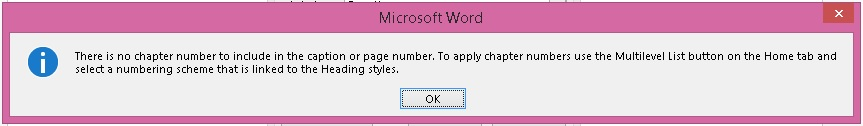
\includegraphics[width=\textwidth]{./Figures/warning.jpg}
     \caption{Insert Caption Warning}
     \label{fig:warning}
 \end{figure}
 \item to fix this we will use SEQ Field, see \footnote{\url{http://gregmaxey.mvps.org/word_tip_pages/seq_field_numbering.html}} for details
 \item you will see something similar to this \{STYLEREF 1 \textbackslash s\}-\{SEQ Equation \textbackslash * ARABIC \textbackslash  s 1 \}, here 1 after STYLEREF referringing to the default Heading 1 style in Word
 \item Replace this 1 with \quotes{ChapterHeading} , Now right click and select Update Field, again right click the field and select Toggle Field Code. This should give you 1-1 
 \item Now set the borders of the table to none
 \item This can be added as a building block now for reuse, Go to Insert Tab, Tables Group, click the table button and select Quick Tables and then Save selection to quick tables gallery, Give it an appropriate name, and choose Equations for Gallery.
 \item Next time whenever you have to insert a new equation go to Insert Tab, the building block we just created will now be listed under Equation Button.
 \end{enumerate}
 \section{Referencing Research Articles}
 This section describes how to use EndNote for citation for research articles.
 Instructions in this handout are carried out using a trial version of EndNote X7 and can be downloaded from \footnote{\url{http://endnote.com/downloads/30-day-trial}}. 
 \subsection{Activity 3: Search for articles online}
 \label{subsec:activity3}
 First we need to search the article to be cited.
 \begin{enumerate}
 \item Start by browsing GoogleScholar \url{https://scholar.google.co.th/}
 \item In the search box enter the title of the paper you want to cite, e.g. \quotes{On convex relaxation of graph isomorphism}
 \item Below the search result click the link \quotes{Cite}
 \item In the resulting Dialog choose APA style
 \item Now click the EndNote link
 \item A file with extension enw will be downloaded, examine the content of the file, for the moment open it with Notepad.
 \item Each entry in the file can easily be guessed.
 \end{enumerate}
 \subsection{Exercise 2: Download 4 more articles }
 Following the procedure in \ref{subsec:activity3} download 4 more EndNote references for the research articles of your area of interest.
 \subsection{Creating EndNote Library}
 An EndNote library is a database containing references to research articles. Let us create one.
 \begin{enumerate}
 \item Click \mystyle{File} menu and then click \mystyle{New}
 \item It will prompt to save the library choose a location give your library a name and click Save
 \end{enumerate}
 \subsection{Importing References in EndNote}
 Follow these steps to Import the downloaded reference files to EndNote:
 \begin{enumerate}
 \item Click \mystyle{File} menu and choose \mystyle{Import} and then \mystyle{File}
 \item Select \mystyle{EndNote Import} in \mystyle{Import File} Dialog, and then click \mystyle{Choose} Button
 \item Select the file you downloaded and click \mystyle{Open}
 \item Finally click the \mystyle{Import} button
 \end{enumerate}
 \subsection{Cite Articles in Microsoft Word}
 Follow these steps to cite articles:
 \begin{enumerate}
 \item Go to \mystyle{EndNote X7} Tab and from \mystyle{Citations} group select \mystyle{Insert Citation}
 \item In the \mystyle{Find field} type any keyword (a word in the title, or name of any author) of the article you need to cite, and click the \mystyle{Find} button
 \item From the search results, click the article you want to cite, and click Insert
 \end{enumerate}
 \subsection{Changing Bibliography Style}
 To apply \mystyle{APA 6th} bibliography style follow these steps
 \begin{enumerate}
 \item Go to \mystyle{EndNote X7} Tab and from \mystyle{Bibliography} group click \mystyle{Style} dropdown
 \item Choose \mystyle{APA 6th} from the list
 \end{enumerate}
 \section{Generating List of Tables/Figures}
 Follow these steps to auto generate list of tables or figures:
 \begin{enumerate}
 \item Go to \mystyle{REFERENCES} tab 
 \item In \mystyle{Captions} group click \mystyle{Insert Table of Figures}
 \item Uncheck \mystyle{Use hyperlinks instead of page numbers}
 \item In the \mystyle{Tab leader} dropdown select \mystyle{none}
 \item In \mystyle{Caption label} dropdown of the \mystyle{General} section choose Table when generating list of tables, and Figure when generating list of Figures
 \item Click OK
 \end{enumerate}
 \subsection{Generating Table of Contents}
 
 \begin{enumerate}
     \item Go to \mystyle{REFERENCES} tab 
     \item In \mystyle{Table of Contents} group click \mystyle{Table of Contents}
     \item Choose \mystyle{Custom table of Contents}
     \item click the \mystyle{Options} button
     \item In the \mystyle{Available styles} under \mystyle{TOC level} remove 1,2 and 3 in front of \mystyle{Heading 1, Heading 2, and Heading 3}
     \item Now enter 1 in front of ChapterTitle style, 2 in front of SectionHeading, and 3 in front of SubSectionHeading \ref{sec:styles}, and click OK button
     \item From Tab leader select none, and uncheck the option User hyperlink instead of page numbers and click OK
 \end{enumerate}